\documentclass[11pt,a4paper]{article}

\usepackage{german,anysize,amsmath,amssymb,amsthm,paralist, array}
\usepackage{url}
\usepackage{dirtree}
\usepackage{enumitem}
\usepackage{color}
\selectlanguage{german}
\usepackage{graphicx}

\usepackage[T1]{fontenc}

\pagestyle{empty}

%\setlength{\textheight}{27cm}
\setlength{\parindent}{0cm}

%enumeration with less space between items
\newenvironment{cEnum}{
\begin{enumerate}
  \setlength{\itemsep}{0pt}
  \setlength{\parskip}{0pt}
  \setlength{\parsep}{0pt}
}{\end{enumerate}}

\begin{document}
\textsc{Technische Universit"at Berlin}{\small\hfill 
Scalable Data Science: Systems and Methods }\\
{\small Database Systems and Information Management Group{\small\hfill WS 2015-2016}\\
C. Boden, S. Schelter, J. Soto, and Prof.~Dr.~Volker~Markl}

\bigskip
\centerline{\Large\textbf{Third Assignment}}
\centerline{\emph{Visualization, PageRank, and Graph Analysis in Apache Flink}}
{\color{red}
\centerline{Due on Monday the 25th of January 2016 at 12:00 noon}
}
\bigskip


\subsection*{I. Exploratory Analysis/Visualization {\color{red}(Total: 4 pts.)}}

In this exercise, you will gain familiarity with the Tableau Desktop software for visualization. To get you started, have a look at their tutorials: http://www.tableau.com/learn/training. Next, you will want to select a dataset (e.g., identify a dataset from the list in my posting on ISIS from a few days ago or choose one of your own). The dataset should be reasonably large (e.g., in the MB to GB range). \\

Once you have identified your dataset, analyze/explore the dataset, prepare a graphic and incorporate appropriate labels, such as the question you aim to answer, the dataset size, and your key findings. Summarize and interpret your findings. Since your dataset may be too large for Tableau feel free to introduce a sampling technique. Select an appropriate sampling cheme, document it, and explore varying samples to show that your findings are consistent. \\

N.B. In general, Tableau generally can produce graphics for up to 1M data points.\\


\subsection*{II. The PageRank Algorithm  {\color{red}(1 pt.)}} 
Compute the PageRank vector for the following graph assuming no taxation. Show your work including the adjacency matrix, the initial PageRank vector, and the values of the PageRank vector for the first three iterations, as well as an approximation of the converged result rounded to two significant figures.

\begin{figure}[h!]
	\begin{center}
		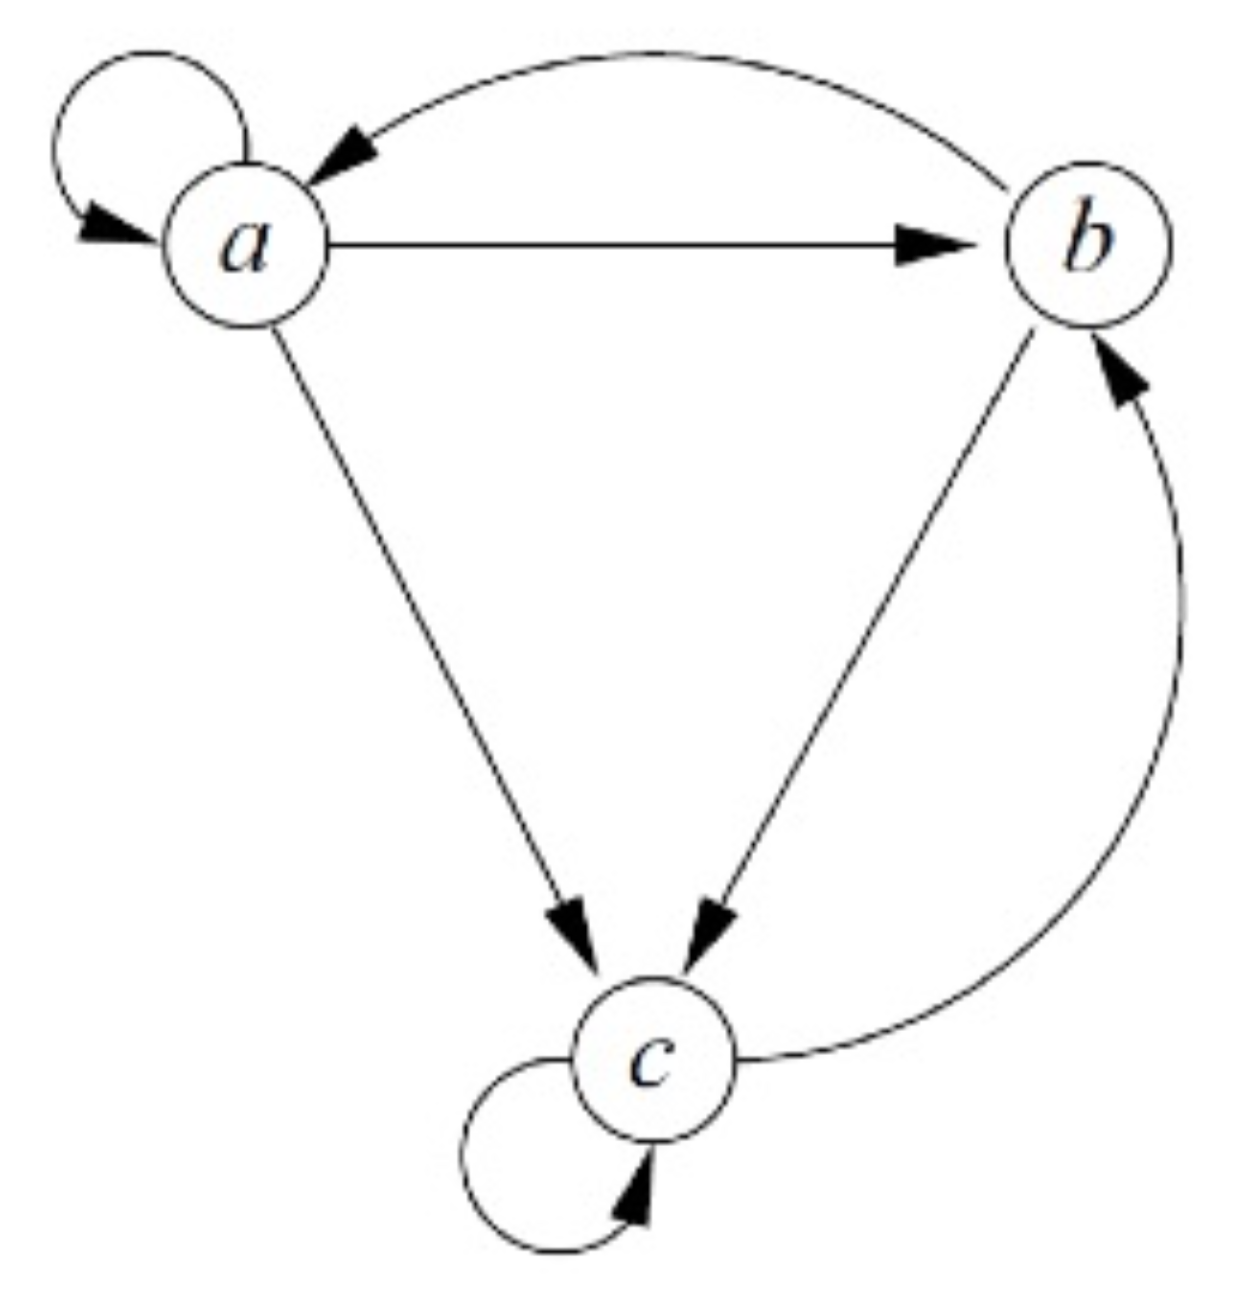
\includegraphics[scale=0.3]{network.png}
	\end{center}
\end{figure}

\subsection*{III. Graph Analysis in Apache Flink {\color{red}(5 pts.)}} 

The Slashdot Zoo dataset represents a signed social network of users of the technology news site Slashdot (slashdot.org), connected by directed ''friend'' and ''foe'' relations. The data set can be found here: \url{http://konect.uni-koblenz.de/networks/slashdot-zoo}. Have a look at the README file to familiarize yourself with the dataset. \\ 

The ''friend'' and ''foe'' labels are used on Slashdot to mark users, and influence the scores as seen by each user. For instance, If user A marks user B as a foe, the score of user B's posts will be decreased as shown to user A. If we consider the direction and add up the incoming and outgoing connections we will obtain two numbers for the degree of the node (i.e., in-degree and out-degree). \\

Use the slashdot-zoo\_stub available at GitLab (as a starting point) and complete it, in order to answer to the following:
\begin{cEnum}
\item Produce a CSV file that contains the overall in-degree distribution. Create the corresponding histogram with appropriate labels, accordingly.
\item Produce a CSV file that contains the overall out-degree distribution. Create the corresponding histogram with appropriate labels, accordingly.
\item Produce a CSV file that contains the out-degree distribution for friend nodes. Create a plot illustrating the probability distribution with appropriate labels, accordingly.
\item Produce a CSV file that contains the out-degree distribution for foe nodes. Create a plot illustrating the probability distribution with appropriate labels, accordingly.
\end{cEnum}

For the latter two items, use a log-log plot and interpret the figures. What is particularly distinctive about them? \\

N.B. The following reference may be of use to you: http://mathinsight.org/degree\_distribution. \\ 
        Lastly, you should ensure that your probability vectors sum to 1. Otherwise, something is not correct.

\newpage
\centerline{\textbf{Deadline and General Instructions}}
\bigskip

For exercise 3, you will want to download the source code stub located here: \\
https://gitlab.tubit.tu-berlin.de/aim3 WS1516/assignments/tree/master/Assignment3\\

Please submit your results to ISIS in a zip archive with the following structure and naming conventions until the above specified deadline: \\

\dirtree{%
 .1 aim3-WS1516-\textless name\textgreater.zip.
 .2 author.txt (contains your name and matriculation number).
 .2 task I.
 .3 the Tableau files.
 .3 the raw data set.
 .2 the graph analysis source codes and CSV files.
 .2 documentation.pdf (answers to the questions posed in each exercise, including the four plots) .
 }

\end{document}